\documentclass[border=10pt]{standalone}
\usepackage{pgfplots}
\pgfplotsset{compat=1.18}

\begin{document}
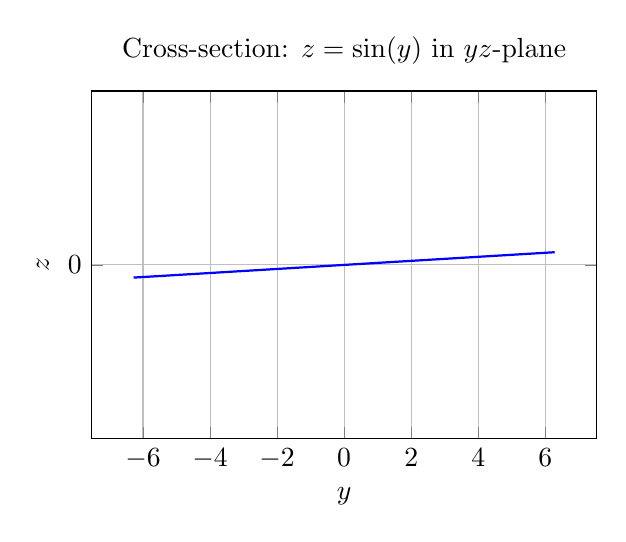
\begin{tikzpicture}
\begin{axis}[
    xlabel={$y$},
    ylabel={$z$},
    title={Cross-section: $z = \sin(y)$ in $yz$-plane},
    grid=major,
    width=8cm,
    height=6cm,
    ymin=-2*pi,
    ymax=2*pi,
    ymax=6.28,
    ymin=-6.28,
    ytick={-6.28, -4.71, -3.14, -1.57, 0, 1.57, 3.14, 4.71, 6.28},
    yticklabels={$-2\pi$, $-\frac{3\pi}{2}$, $-\pi$, $-\frac{\pi}{2}$, $0$, $\frac{\pi}{2}$, $\pi$, $\frac{3\pi}{2}$, $2\pi$},
    ymax=1.5,
    ymin=-1.5,
]
\addplot[
    domain=-2*pi:2*pi,
    samples=100,
    thick,
    blue,
] {sin(x)};
\end{axis}
\end{tikzpicture}
\end{document}